\documentclass[12pt,twoside]{book}
\usepackage[british]{babel}
\usepackage[utf8]{inputenc}

\usepackage[a4paper,
			lmargin=1.5in,
			vscale=0.8]{geometry}

\usepackage{amsmath}
\usepackage{graphicx}
\usepackage{parskip}
\usepackage{natbib}
\usepackage{pgfgantt}
\usepackage{lscape}
\usepackage{pdfpages}
\usepackage{graphicx}
\usepackage{xcolor}
\usepackage[listingsutf8,minted]{tcolorbox}
\usepackage{hyperref}
\usepackage[chapter]{tocbibind}
\usepackage{doc}
\usepackage{minted}
\usepackage{listings}
\usepackage{listingsutf8}
\usepackage[colorinlistoftodos]{todonotes}

\usepackage{fontawesome}

\usepackage{tikz}
\usetikzlibrary{trees}


\begin{document}

\frontmatter
%!TeX root=Dissertation.tex

\begin{titlepage}
\Large
A Report submitted in partial fulfilment of\\
 the regulations governing the award of
\par
the Degree of\\[5mm]
{\huge	 BSc (Honours) Programme Name }\\[5mm]
at the University of Northumbria at Newcastle
\par
\vspace*{1in}
{\Large Project Report}
\par\vspace{1em}
{\Huge \bfseries Your Project Title}
\vfill
Your Name
\par\vspace{1em}
2016/ 2017
\par\vspace{1em}
General Computing/Software Engineering Project
\end{titlepage}

%!TeX root=Dissertation.tex

\chapter{Declaration}

I declare the following:

\begin{enumerate}

\item that the material contained in this dissertation is the end result of my own work and that due acknowledgement has been given in the bibliography and references to ALL sources be they printed, electronic or personal.

\item the Word Count of this Dissertation is $\langle\mathrm{len}\rangle$\\
(result of shell command \mintinline{bash}{texcount -total -inc Dissertation.tex})

\item that unless this dissertation has been confirmed as confidential, I agree to an entire electronic copy or sections of the dissertation to being placed on the eLearning Portal (Blackboard), if deemed appropriate, to allow future students the opportunity to see examples of past dissertations.  I understand that if displayed on eLearning Portal it would be made available for no longer than five years and that students would be able to print off copies or download. 

\item I agree to my dissertation being submitted to a plagiarism detection service, where it will be stored in a database and compared against work submitted from this or any other School or from other institutions using the service. 

In the event of the service detecting a high degree of similarity between content within the service this will be reported back to my supervisor and second marker, who may decide to undertake further investigation that may ultimately lead to disciplinary actions, should instances of plagiarism be detected.

\item I have read the Northumbria University/Engineering and Environment Policy Statement on Ethics in Research and Consultancy and I confirm that ethical issues have been considered, evaluated and appropriately addressed in this research.
\end{enumerate}
\vspace{1in}
\large{SIGNED:\dotfill}

%!TeX root=Dissertation.tex

\chapter{Acknowledgements}

%!TeX root=Dissertation.tex

\chapter{Abstract}

A summary of the entire project.
From background to conclusions.
I recon on about half a page as the upper end of the summary.

This is an example structure for the Terms-of-Reference and the Dissertation.
Along with some notes.

You can start by forking the repository on github
\url{https://github.com/dr-alun-moon/cs-dissertation}.  Then you have a working copy of this document as a starting point.

\tableofcontents

\mainmatter
%!TeX root=Dissertation.tex

\chapter{Introduction}
This document is split into several files.  This makes the editing easier, if the file management a little harder.

The two principle means of including sub parts into a main document are the \LaTeX\ commands \verb"\input" and \verb"\include"
\section{Splitting the Input}
\paragraph{The input command } simply reads that file in, at that point in the main file.  The result is as if the inputed file was pasted in at the point of the command.

\paragraph{The include command} is a little more complex.  The main point to note is that it forces a new page, then reads in the file.  It is good foe content that needs to start a fresh page, such as chapters.  As a rule of thumb I put each chapter in an included file.

\subsection{Some tricks.}  The Dissertation uses the book class, that gives the Chapter as the top sectional element, followed by section, subsection, paragraph.   The Terms-of-reference uses the article class, which starts at the section level.

By writing the ToR as a driver document that handles all the setting up, and then inputing the tor content from a separate file.  When it comes to including the tor as an appendix in the dissertation, you can start a chapter then just input the tor content file.

\begin{tcblisting}{listing only}
    \appendix
    \chapter{Terms of reference}
    %!TeX root=TermsOfReference.tex

\section{Background}
The modern technological landscape demands much from innovation. 
We must find new ways of solving existing and new problems in the world. 
This is amazing for convenience, and quality of life, but does pose a problem for security. 
There is Hypponen's law in IOT that states, the more you add in terms of functionality, the more that must be secured. \citep{hypponen}
A concrete cube may be secure, but is not overly functional. I am incredibly interested in the duality between attack and defence. 
It seems to be a constant cat and mouse game of which defence is paramount. \citep{cutandmouse}
I hope that by looking at both sides with a purple team perspective, I can gain a deep understanding of the landscape we have currently and moving forwards. 

Cyber-Security is really "Managed insecurity", I intend to discover where cyber attacks are at, and how they have innovated over the years.
Cyber threats are growing, how can be detect them? How can we proactively block them? These are questions that must be answered in order to get a good overview.
I must be able to show my understanding in a theoretical and practical way to be able to potentially apply it to a real life scenario. 
I will have to develop my understanding of infrastructure, networking, semi low-level programming and penetration testing.

Developing realistic solutions for smaller businesses is really important. They are arguably more at risk, with less resources for security. \citep{sme}
The is a culture of security snake-oil and scare-ware, and supposed all-in-one solutions rather than defence-in-depth. This is evident in the numerous adverts that claim much and deliver little. \citep{SnakeOil}
With the detection work, I hope to show the importance of the human element to security, how it can be the weakest link, or the strongest asset.  \citep{humanFactor}
I must look at current solutions with a critical eye with care to be realistic about defence. 

Malware has evolved over time, what was once an exercise of what was possible, is now a platform for theft and crime. \citep{malwareHistory}
Defences catch up over time, it will be eye-opening to see the different methods historically that the two sides try to out-smart each other. \citep{malwareHistory}
Malware analysis is something I haven't really touched on before, though I have be interested for a long while now. It will benefit my defence greatly.


\section{Proposed Work}
\label{proposed}
I aim to create documentation in the form of my dissertation to describe the Cyber-Security landscape in regards to infrastructure. 
This will involve talking about infrastructure directly, it's use, implementation and potential pitfalls, but more importantly, how it can be secured.
On the other side, I will be looking at the common ways that infrastructure is compromised, in a network setting. 
I do think that a good comparison is important for this. The dissertation will have the approach of being an overview, as I feel that is the best way to cover the bigger picture. 
I will go into relative depth where it is nessesary. The experiment will simply just compare a set of attacks to a set of defences, with analysis of the results. Details will come in the synthesis, as
it entirely depends on my research to which exact direction I go in. 

I will be investigating how threats have evolved as a whole, talking about malware mechanisms, obfuscation and clever exfiltration. 
I believe it is important to at least touch on how this was done in the past, 
to understand how the future may follow similar foundations. Naturally an investigation into threats would be pointless without a practical defence, 
I hope to compare both endpoint and infrastructure defences in relation to both a sample of threats, and to one another. I will then analyse this data and draw sensible conclusions based upon it.

I also hope to create a rudimentary intrusion detection system written in C. This will be a proof of concept to show my understanding, rather than a product. My hopes are that by developing network defence myself, 
I can gain an even deeper understanding. It will also illustrate the scale that corporate products can run at, including extra methods that are out of scope for me.
This is secondary to the main experiment. 

\section{Aims and Objectives}
\subsection{Aims}
\begin{quote}
	To understand the theory behind defence in relation to common threat vectors.
	To develop attack and defence skills to aid the theory, in a practical manner.
\end{quote}

\subsection{Objectives}
\begin{enumerate}
	\item \textbf{Analysis of historic threats and malware}
	\item \textbf{Analyse modern attack:defence landscape}
	\item \textbf{Analysis of defence technologies}
	\item \textbf{Explanation of entry vectors and profiling}
	\item \textbf{Explanation of exploitation}
	\item \textbf{Explanation of obfuscation}
	\item \textbf{Explanation of exfiltration}
	\item \textbf{Investigate IDS/IPS systems w/ comparison}
	\item \textbf{Illustrate proof of concept IDS}
	\item \textbf{Investigate antivirus systems w/ comparison}
	\item \textbf{Discussion of meaningful defence}
\end{enumerate}

\subsection{PoC IDS Objectives (It must..)}
\begin{enumerate}
	\item \textbf{Detect network interfaces}
	\item \textbf{Bind to a network interface}
	\item \textbf{Capture data and output to a file/standard output}
	\item \textbf{Flag up unusual activity from a few notable attack types}
	\item \textbf{Control via command switches}
	\item \textbf{Be well written and meaningful to the idioms of the language}
	\item \textbf{Have testing/design documentation}
	
\end{enumerate}

\section{Skills}
\begin{enumerate}
	\item [$\bullet$] Programming in C (KF5006)
	\item [$\bullet$] Networking Technology 3 (KF6005)
	\item [$\bullet$] Advanced Operating Systems II (KF6003)
	\item [$\bullet$] Cyber-Security Awareness
	\item [$\bullet$] Reverse-Engineering
	\item [$\bullet$] Data Analysis
\end{enumerate}

\section{Resources}
\subsection{Hardware}
\begin{description}
	\item[$\bullet$] Dedicated high RAM machine - Already bought
	\item[$\bullet$] Lab Machines for possible testing
\end{description}

\subsection{Software}
\begin{description}
	\item[$\bullet$] VMware Workstation - To host vulnerable and attacker infrastructure
	\item[$\bullet$] VScodium - IDE for IDS development
	\item[$\bullet$] Packet Libraries - unsure about specifics at the time of writing, likely scapy and libpcap
	\item[$\bullet$] Various Antivirus Licences - Prefer free or monthly subscription
	\item[$\bullet$] IDS/IPS/SIEMs Licences - Will have to prefer free or cheap ones (as a small company would)
	\item[$\bullet$] Malware Samples - Sourced from Github collections
	\item[$\bullet$] Operating System Distributions - Obtained online 
\end{description}

\section{Structure and Contents of the Report}
\subsection{Planned Report Structure (Order may change)}


\paragraph{Introduction} - This chapter sets out the basis of the project, the motivations behind it and what I am looking to investigate. 
It will summarise the whole project.

\paragraph{Analyse historic \& modern defence} - This chapter is a broad overview of the cat and mouse game, with a focus on how both sides evolve over time, 
and how to tip the scales in the defences favour. Analysis of defence technologies directly after (Anomaly Detection, signature matching, whitelisting etc..). 

This chapter then covers cases of past incidents, how they happened, why they were effective and what we can learn from them for modern day. 
I will cover an assortment of notable malware. History and modern may be split into two paragraphs.

\paragraph{Explanation of entry points and profiling} - This chapter covers the idea of what a vulnerability is at it's core, how they are found
and the commonalities among vulnerabilities. It will include the discussion of common pen-testing tools for the enumeration/scanning phase.
Additonally I will look at common attack vectors for malware to get in.

\paragraph{Explanation of malware mechanisms} - This chapter covers the common mechanisms of exploitation and stealth that malware makes use of. 
This includes the use of obfuscation, encryption, exfiltration and the impacts they have. This covers a description of the methods, rather than ouright historic implementation.
May be split into their own sections/chapters for the sake of detail.


\paragraph{Investigate antivirus systems w/ comparison} - This chapter is to lay out my experiment methodology, why I did what I did, what I'd expect vs what I got and an analysis of the results themselves.  A sample of threats/malware may be tested.

\paragraph{Investigate IDS/IPS systems w/ comparison} - This chapter is to lay out my experiment methodology, why I did what I did, what I'd expect vs what I got and an analysis of the results themselves. A sample of threats/malware may be tested.

\paragraph{Proof of Concept IDS} - I will talk about what can be learned from it, in relation to the scale of commercial products, along with the technologies used.


\paragraph{Discussion of meaningful defence} - This chapter encompasses what can be done to aid defence to it's maximum. I will focus on defense in depth and diversification of defence mechanisms. 
Topics include, proper training, access control, security positive culture, adequate funding, regular security testing, development infrastructure and a wide variety of hardware solutions. 
Will likely be split into sub paragraphs and sections as it's a vast topic.

\subsection{Conclusion} This will summarise all that was found, how it relates to what I set out to discover and what it means for the future of defence. 


\subsection{List of Appendices}
\begin{itemize}
	\item ToR
	\item Experiment and PoC Design/Testing
	\item IDS Source Code
	\item Experimentation Result Documentation
	\item Risk Assessment
	\item Ethics Form (Depending on ethics approval process)
\end{itemize}

\section{Marking Scheme}
The marking scheme sets out what criteria we are going to use for the project.

\paragraph{Project Type:} General Computing

\paragraph{Project Report}
\subparagraph{Analysis}
\begin{itemize}
	\item Analyse historic \& modern attack/defence landscape - Analysis of literature & malware/threats 
	\item Explanation of entry vectors and profiling
	\item Explanation of malware mechanisms
\end{itemize}

\subparagraph{Synthesis}
\begin{itemize}
	\item Investigate antivirus systems w/ comparison
	\item Investigate IDS/IPS systems w/ comparison
	\item Illustrate proof of concept IDS \& implementation of technologies
\end{itemize}

\subparagraph{Evaluation}
\begin{itemize}
	\item Discussion of meaningful defence
\end{itemize}

\paragraph{Product}
\begin{itemize}
	\item Dissertation Paper
	\item Experiment and PoC Design/Testing
	\item IDS Source Code
	\item Experimentation Result Documentation w/ Metric Justification
\end{itemize}

\subparagraph{Fitness for Purpose}~
\begin{itemize}
	\item There must be analysis of both sides
	\item There must be comparison of feasible solutions
	\item The program must be functional to a proof of concept level
\end{itemize}

\subparagraph{Build Quality}~
\begin{itemize}
	\item Experiment design quality
	\item Code quality \& testing
	\item Quality of analysis \& synthesis
	\item Quality of meaningful mitigation
\end{itemize}
\section{Project Plan}
\noindent
\rotatebox{90}{%!TeX root=TermsOfReference.tex

% A lot of the settings here are tuned to fit a landscape gantt chart into
% an A4 piece of paper.
\begin{ganttchart}[
time slot format=little-endian,
calendar week text=\currentweek,
x unit=2.4pt,
y unit chart=14pt,
y unit title=12pt,
title label font=\scriptsize,
bar top shift=.15,
bar height=0.7,
milestone label font = \small,
group label font = {\tiny\bfseries},
group inline label node/.append style=centered,
hgrid=true,vgrid={*6{draw=none},dotted},
region/.style={inline,group peaks width=2,
  group peaks height=0.25, group height=0.5,
  group top shift=0.2 ,group/.append style={fill=#1}},
milestone left shift=0,
milestone right shift=1,
ms/.style={inline,
    milestone inline label node/.append style={#1=0pt}}
]%
% For semester dates see
% https://www.northumbria.ac.uk/about-us/university-services/academic-registry/registry-records-and-returns/academic-calendars/
{21/9/20}{28/05/21} %<- Dates Gantt Chart runs from and to

\gantttitlecalendar{year,month,week=1}\\

% Highlight Semsters and Vactions
\ganttgroup[region=blue!20]{Semester 1}{21/9/20}{22/1/21}
\ganttgroup[region=blue!50]{Semester 2}{18/1/21}{28/5/21}\\
\ganttgroup[region=red!50]{Christmas}{21/12/20}{8/1/21}
\ganttgroup[region=green!25]{Easter}{29/3/21}{16/4/21}\\

% Project Deadlines (from the Project Handbook)
\ganttmilestone[ms=left]{PID}{12/10/20}
\ganttmilestone[ms=left]{final \bfseries TOR}{16/11/20}
\ganttmilestone[ms=right]{Analysis}{25/12/20}
\ganttmilestone[ms=left]{Synthesis}{22/02/21}
\ganttmilestone[ms=left]{Evaluation}{19/03/21}
\ganttmilestone[ms=left,milestone/.append style={fill=red}]{\bfseries Submit}{29/4/21}
\ganttnewline[thick]

% --Tasks go here
% put in a title, a start date, end date...
\ganttbar{TOR}{28/9/20}{26/10/20}
\ganttbar[inline]{\emph{revise}}{28/10/20}{16/11/20}\\
\ganttnewline[thick]

%\ganttbar{Analysis}{27/10/20}{25/12/20}
\ganttbar{Defence Tech (Obj \ref{talkDefenceTech})}{5/10/20}{15/10/20}\\
\ganttbar{Entry Vector (Obj \ref{talkEntryVectors})}{16/10/20}{23/10/20}\\
\ganttbar{History (Obj \ref{talkHistory})}{24/10/20}{30/10/20}\\
\ganttbar{Modern (Obj \ref{talkModern})}{31/10/20}{07/11/20}\\
\ganttbar{Exploitation (Obj \ref{talkExploitation})}{08/11/20}{20/11/20}\\
\ganttbar{Obfuscation (Obj \ref{talkObfuscation})}{21/11/20}{30/11/20}\\
\ganttbar{Exfiltration (Obj \ref{talkExfil})}{1/12/20}{10/12/20}\\
\ganttnewline[thick]

%\ganttbar{Synthesis}{26/12/20}{10/02/21}
\ganttbar{Attack Lab (Obj \ref{makeLab})}{26/12/20}{10/01/21}\\
\ganttbar{PoC Build (Obj \ref{write-code})}{11/01/21}{25/01/21}\\
\ganttbar{IDPS Compare (Obj \ref{compareIDPS})}{26/01/21}{10/02/21}\\
\ganttbar{AV Compare (Obj \ref{compareAV})}{11/02/21}{22/02/21}\\
\ganttnewline[thick]

%\ganttbar{Evaluation}{11/02/21}{15/03/21}
\ganttbar{Defence-In-Depth (Obj \ref{talkDefenceInDepth})}{23/02/21}{10/03/21}\\
\ganttbar{Evaluation Of Project}{11/03/21}{19/03/21}\\
\ganttnewline[thick]

\ganttbar{Finalise \& Refine}{20/03/21}{28/04/21}

\end{ganttchart}
}

%order may change - Some sections will relate on one another, for example, when analysing malware, I may reference later in the paper to a discussed topic. 
% I will move sections accordinly, but I have to keep to the overall structure so referencing may be needed
\end{tcblisting}

\section{Magic comments}
Since \LaTeX\ needs to have a certain amount of setup (known as the preamble), this is the file that needs to be build.  From a Makefile or command-line, this is simple enough.

Several editors allow you to trigger the build from within their environment.  Here the file you are editing is a subpart and not the mater document that needs to be passed to \LaTeX.   The editor needs to know which \path{.tex} file is the master document.  Some editors recognise a magic comment placed at the top of a sub-file.
\begin{tcblisting}{listing only}
%!TeX root=Dissertation.tex
\end{tcblisting}
This informs the editor that \path{Dissertation.tex} is the file to build to rebuild the document.  I can save changes and just press the key combination set to trigger a \LaTeX\ build, and the editor knows how to do the rest.

\part{Analysis}
%!TeX root=Dissertation.tex

\chapter{Some Literature}

Dario Taraborelli, has written a nice page illustrating some of \href{http://nitens.org/taraborelli/latex}{The Beauty of LaTeX} illustrating some of the finer points of TeX et.al. typesetting

\url{TeXample.net} is a site that has many spectacular examples\footnote{\url{http://www.texample.net/tikz/examples/}} of graphics creation in LaTeX. It mainly illustrates the use of the tikz package.

Two web sites provide forums for questions and answers on latex. \href{http://www.latex-community.org/}{LaTeX Community} and \href{http://tex.stackexchange.com/}{TeX - LaTeX Stack Exchange}

\section{References and searching}

\LaTeX\ and \BibTeX\ provide excellent support for referencing and citations (especially with natbib\footnote{see online manual at \url{http://mirror.ox.ac.uk/sites/ctan.org/macros/latex/contrib/natbib/natbib.pdf} or with the command \texttt{texdoc natbib}}).  Getting your .bib file populated with material can be time consuming. Among the many ways of doing this are:
\begin{itemize}
\item    Search engines like the University Library allow you to export your saved searched in a bibTeX file
\item    Google scholar https://scholar.google.co.uk/ have an option to create the BibTeX entry for results.
\item    Zotero provides a plugin for Firefox, that extracts information from a web page and exports a bibTeX file. (Great for getting references to Wikipedia, or getting book details from Amazon)
\end{itemize}

These are great, but sometimes the bibTeX file needs a little post-editing. Usually I end up deleting extraneous fields and escaping TeX characters if needed.

\begin{enumerate}
\item Search for articles, books etc, grab the bibTeX file,
\item \verb"\backslash cite{}"and use
\item \verb"\bibliography{save1,litrev,canon}" with
\item \verb"\bibliographystyle{plainnat}" (having \verb"\usepackage{natbib}" in the preamble)...
\end{enumerate}
 Harvard referencing of your material... job done

 \section{Writing your dissertation}
 
The most valuable document is the \emph{Project Handbook}, this gives guidance
on the structure and contents of the Terms-of-Reference and Dissertation.  It
also has the marking scheme, which is an important read as this describes what
we are looking for when marking the project.

\subsection{The Logbook}
Use your logbook and a project diary, make notes of what you do as you do
them.  As questions arise, make a note of them at the time, and then you are
ready for the weekly meeting.

In the meeting make notes of whet we discuss for the week ahead, and issues
that come up that can be looked at later.

Some students in the past have kept a project blog.

\subsection{The Dissertation} 
There are several good sites about with advice on how to write clearly.  Not
all of the advice is directly relevant to writing a B.Sc dissertation in
Computer Science.  The advice may not even be consistent, 

William Stallings \citep{Stallings} maintains a good website of resources for
Computer science students.


%!TeX root=Dissertation.tex

\chapter{Tools}

\section{\LaTeX}
I recommend the \TeX live distribution, which can be downloaded from
\url{https://www.tug.org/texlive/}.  There are installation packages for Windows, Linux, and Macs here.  For Linux machines there is often a copy of texlive in the package repository.

\begin{figure}[h]
\begin{minted}{bash}
apt search texlive
\end{minted}
    \caption{Searching for texlive on Debian/Ubuntu systems}
    \label{}
\end{figure}
\emph{Edit 2018\/} on my machine at work I've dropped the Ubuntu version of
texlive as it didn't pull in all the documentation for the packages (see section
\ref{tex:texdoc})
\section{Editors}
Any text editor will do.   I wrote my MSc dissertation in \texttt{vi}\footnote{\url{https://en.wikipedia.org/wiki/Vi}}
\footnote{Hardcore Unix use}!  I've gone full circle and returned to using
\texttt{vi} for latex at work and at home.

In practice, many modern editors have a rich set of tools to help with the editing process.  From syntax-highlighting, auto-completion, to rebuilding.

\subsection{My setup}
Currently I'm using \texttt{vim} to edit this document, and \texttt{latexmk} to
build  the pdf.   I've two terminals open, in one I have the editor and the
other the command
\begin{minted}{bash}
letexmk -pdf -pvc -latexoption=-shell-escape Dissertation
\end{minted}

The options are
\begin{description}
	\item[\texttt{-pdf}] makes sure a pdf is generated via \texttt{pdflatex}
	\item[\texttt{-pvc}] monitors the \texttt{.tex} files and reruns the build
		process if changes are made, it automatically opens and updates the pdf
		viewer as needed.
	\item[\texttt{-latexoption=-shell-escape}] because I'm using the
		\texttt{minted} package for syntax highlighting, the
		\texttt{-shell-escape} option is passed on to \texttt{pdflatex}.  Minted
		uses pygmentize as an external program to perform the highlighting.
\end{description}
		
\subsection{Vi/Vim+vimtex}
Vim \url{https://www.vim.org/} the modern incaration of \texttt{vi} has an
extension package \texttt{vimtex} \url{https://github.com/lervag/vimtex}.
I'm finding these more than adequate for my editing needs.  Vi is part of the
POSIX standard and is either going to be installed or very easy to install on
any Unix like system. Windows users have several choises on how to use vim and
latex.

\subsection{Atom}
As it is a very extensible editor, there are a number of add-ons that help with latex.

\begin{description}
    \item[language-latex] \url{https://atom.io/packages/language-latex} which provides syntax highlighting.
    \item[latex] \url{https://atom.io/packages/latex} which provides means of compiling latex documents from within the editor.
    \item[pdf-view] \url{https://atom.io/packages/pdf-view} which is a PDF viewer.  (I'm not sure about this one, I can't tell if it is too much of a strain on the editor)
\end{description}

\subsection{TeXworks and TeXShop}
The TeXShop editor on the Mac inspired TeXworks on Windows.  This is a nice little editor with a good pdf previewer built in.

\subsection{Texmaker}
    This looks like a nice clean editor for LaTeX.  It has  usefull pallets of commands.
\subsection{TeXnicCenter}
    An editor with a lot of tools.
    A  capable system.
\subsection{Online}
Two online web based editing web-applications are
\begin{itemize}
  \item ShareLaTeX \url{https://www.sharelatex.com/}
  \item Overleaf  \url{https://www.overleaf.com/}
\end{itemize}

\section{PDF viewers}
Latex generates pdf files out of the box.  There are some good PDF viewers about.  The ones below integrate nicely with the Atom latex tools.
\subsection{Skim -- OSX}
The viewer for Macs \url{http://skim-app.sourceforge.net/}.
\subsection{Sumatra PDF -- Windows}
A good viewer for Windows based machines\\ \url{https://www.sumatrapdfreader.org/free-pdf-reader.html}.

\paragraph{A note about Adobe Acrobat on  Windows machines.}
On windows machines Acrobat locks the file when it opens it, this means that pdflatex and tools cannot write to the file to rebuild it.

\section{SyncTeX integration}
In the settings for the latex plugin for Atom, and the various PDF viewers, you'll see settings for something called SyncTeX.  This does two useful things.

\emph{Firstly} it allows the editor to move the document to the position the cursor is at in the text.  In Skim and Sumatra the viewer displays a coloured dot corresponding to the position of the cursor.

\emph{Second and more useful} is allows the PDF viewer to control the cursor position int he editor.  Click on a location in the PDF, and the cursor in the editor is moved to the corresponding file and location in the sources.

\section{GitHub}
\emph{Treat the documents as code.}
Put the ToR and Dissertation under version control.  It also makes moving your work between university and home easy.  Just commit all the changes, push the repository back to the server, then pull the repository at the other end.  It also means you have a copy backed up.

\paragraph{Sign up for the Student Developer Pack} See \url{https://education.github.com/} and \url{https://education.github.com/pack/}.  They will give you unlimited private repositories (normally \$7/month) while you are a student.

\section{Perl}\label{perl}
Some of the \emph{very} useful tools in texlive, need a Perl installation to work.   In Linux and Macs, perl should be there automatically.  For windows although texlive does install a minimal Perl set, it isn't enough for the really usefull tools (see \ref{latexmk} and \ref{texcount}).

\paragraph{On Windows machines install Perl before TeXlive.}
Make sure that the \path{Perl.exe} is in the system PATH before installing TeXlive.   My Windows installation of Perl is Strawberry Perl \url{http://strawberryperl.com/}.


\section{TeXlive utilities}
There are a couple of very utilities that come with TeXlive, they do need a complete Perl installation (see \ref{perl}).

\subsection{latexmk}\label{latexmk}
Latex needs several passes through to collate and use cross references.  It also needs a pass by BibTeX to compile the reference list, and latex passes to put the citations in.

\texttt{latexmk} is a make like program that understands latex, it can parse the log files generated and re-run the appropriate tools until a build is complete.
\begin{tcblisting}{listing only, listing options={language=bash}}
    latexmk -pdf TermsOfReference
\end{tcblisting}

\subsection{texcount}\label{texcount}
\texttt{texcount} parses the docment, following any inputed or included files, and counts the words used.  Being TeX aware it knows how to ignore the markup.
\begin{tcblisting}{listing only, listing options={language=bash}}
    texcount -total -inc Dissertation.tex
\end{tcblisting}

\subsection{texdoc}\label{tex:texdoc}
Latex is \emph{very} well documented.  To find the documentation for a package, which are loaded in the preamble.  Use \texttt{texdoc} with the package name.
\begin{tcblisting}{listing only,listing options={language=bash}}
    texdoc minted
    texdoc tcolorbox
    texdoc tikz
\end{tcblisting}

\section{Listings}
There are several packages that layout code listings, complete with syntax highlighting.  Their advantage is that they can read in and highlight a source-file in the appropriate language.


\subsection{minted}
I use the \texttt{minted} package,  it does require the use of an external program.  You will need to have Pygments \url{http://pygments.org/} installed, which depends on having a Python installation \url{https://www.python.org/}.

\begin{tcblisting}{}
\inputminted{c}{hello.c}
\end{tcblisting}

In running latex you'll need to enable shell-escape.
\begin{tcblisting}{listing only}
pdflatex -shell-escape Dissertation
latexmk -latexoptions=-shell-escape Dissertation
\end{tcblisting}
Or see the settings for the latex Atom package

\subsection{listings}
Listings is an older package.  It doesn't produce coloured output, but it is written in tex, so it has no external dependencies.
\begin{tcblisting}{}
\lstset{language=c}
\lstinputlisting{hello.c}
\end{tcblisting}


\part{Synthesis}
%!TeX root=Dissertation.tex

\chapter{Some TeXnical Details}

\section{Structure of the file set}
The Terms of Reference and Dissertation are split into several files, to ease
editing, and exploit some of \LaTeX's capabilities.
The structure is relatively \emph{flat} with little hierarchy of directories,
directories and sub-directories can be added to simplify some of the structure
as the project grows.

The principle files are:

\paragraph{\texttt{Makefile}} I use \texttt{make} still as my build driver.
Any automated build system can work with \LaTeX\ files, it just needs to know
that PDFs are build from \texttt{.tex} files.

\paragraph{\texttt{TermsOfReference.tex}} This is the main file for creating
the \emph{Terms of Reference}.  It pulls in the \texttt{tor.tex} file, the
Gantt chart from \texttt{gantt.tex}, and the ethics and risk assessment forms
from scanned PDFs.  The document is typeset as an \texttt{article}.

\paragraph{\texttt{Dissertation.tex}} Is the main file for creating the
dissertation.   This pulls in a number of other files as required.	
It is typeset as a \texttt{book}.  The sectioning starts as \verb'\chapter'
and has \verb'\section'  within.  This way the terms of reference can be
included as a chapter in the appendix.
The chapters are each included using \verb'\include',  this allows the
chapters to be written as separate files.  The difference between
\verb'\include' and \verb'\input' is that \verb'\include' forces a new
right-hand page to start (good for starting chapters).

\subsection{Subsidiary files}
\paragraph{\texttt{tor.tex}} This file is the main \emph{Terms-of-Reference}
file.  By using \verb'\input' in the  \texttt{TermsOfReference.tex} document,
this gets included and typeset.  

\paragraph{\texttt{gantt.tex}} The Gantt chart is a little complex, so gets
put into a separate file, see section \ref{gantt-chart}.

\subsection{The Gantt Chart}\label{gantt-chart}
The Gantt chart in the Terms-of-Reference is drawn with another latex package.
It uses an \texttt{input} command to pull it into the tor (and dissertation).

Most of the file \path{Gantt.tex} is the setup of the Gant chart, in order to
make it fit in one page.  The bottom section is where you can define the
tasks.
Each bar has a title, a start date, and an end date.  Milestones have a title
and a date.  The \texttt{ms} option can be set to left or right to control
which side of the milestone mark the text label.

\begin{tcblisting}{listing only}
% --Tasks go here
% put in a title, a start date, end date...
 \ganttbar{TOR}{11/9/17}{13/10/17}
 \ganttbar[inline]{\emph{revise}}{15/10/17}{10/11/17}\\
 \ganttbar{Analysis}{18/9/17}{24/11/17}\\
 \ganttbar{Design}{31/10/17}{17/1/18}
 \ganttmilestone[ms=right]{Build complete (Obj \ref{write-code})}{18/1/18}\\
 \ganttbar{Exploration}{22/9/17}{15/11/17}
%
\end{tcblisting}


\part{Evaluation}


\bibliographystyle{plainnat}
\bibliography{c,unix,writing,latex}

\part{Appendices}
\appendix

\chapter{Terms of Reference}
%!TeX root=TermsOfReference.tex

\section{Background}
The modern technological landscape demands much from innovation. 
We must find new ways of solving existing and new problems in the world. 
This is amazing for convenience, and quality of life, but does pose a problem for security. 
There is Hypponen's law in IOT that states, the more you add in terms of functionality, the more that must be secured. \citep{hypponen}
A concrete cube may be secure, but is not overly functional. I am incredibly interested in the duality between attack and defence. 
It seems to be a constant cat and mouse game of which defence is paramount. \citep{cutandmouse}
I hope that by looking at both sides with a purple team perspective, I can gain a deep understanding of the landscape we have currently and moving forwards. 

Cyber-Security is really "Managed insecurity", I intend to discover where cyber attacks are at, and how they have innovated over the years.
Cyber threats are growing, how can be detect them? How can we proactively block them? These are questions that must be answered in order to get a good overview.
I must be able to show my understanding in a theoretical and practical way to be able to potentially apply it to a real life scenario. 
I will have to develop my understanding of infrastructure, networking, semi low-level programming and penetration testing.

Developing realistic solutions for smaller businesses is really important. They are arguably more at risk, with less resources for security. \citep{sme}
The is a culture of security snake-oil and scare-ware, and supposed all-in-one solutions rather than defence-in-depth. This is evident in the numerous adverts that claim much and deliver little. \citep{SnakeOil}
With the detection work, I hope to show the importance of the human element to security, how it can be the weakest link, or the strongest asset.  \citep{humanFactor}
I must look at current solutions with a critical eye with care to be realistic about defence. 

Malware has evolved over time, what was once an exercise of what was possible, is now a platform for theft and crime. \citep{malwareHistory}
Defences catch up over time, it will be eye-opening to see the different methods historically that the two sides try to out-smart each other. \citep{malwareHistory}
Malware analysis is something I haven't really touched on before, though I have be interested for a long while now. It will benefit my defence greatly.


\section{Proposed Work}
\label{proposed}
I aim to create documentation in the form of my dissertation to describe the Cyber-Security landscape in regards to infrastructure. 
This will involve talking about infrastructure directly, it's use, implementation and potential pitfalls, but more importantly, how it can be secured.
On the other side, I will be looking at the common ways that infrastructure is compromised, in a network setting. 
I do think that a good comparison is important for this. The dissertation will have the approach of being an overview, as I feel that is the best way to cover the bigger picture. 
I will go into relative depth where it is nessesary. The experiment will simply just compare a set of attacks to a set of defences, with analysis of the results. Details will come in the synthesis, as
it entirely depends on my research to which exact direction I go in. 

I will be investigating how threats have evolved as a whole, talking about malware mechanisms, obfuscation and clever exfiltration. 
I believe it is important to at least touch on how this was done in the past, 
to understand how the future may follow similar foundations. Naturally an investigation into threats would be pointless without a practical defence, 
I hope to compare both endpoint and infrastructure defences in relation to both a sample of threats, and to one another. I will then analyse this data and draw sensible conclusions based upon it.

I also hope to create a rudimentary intrusion detection system written in C. This will be a proof of concept to show my understanding, rather than a product. My hopes are that by developing network defence myself, 
I can gain an even deeper understanding. It will also illustrate the scale that corporate products can run at, including extra methods that are out of scope for me.
This is secondary to the main experiment. 

\section{Aims and Objectives}
\subsection{Aims}
\begin{quote}
	To understand the theory behind defence in relation to common threat vectors.
	To develop attack and defence skills to aid the theory, in a practical manner.
\end{quote}

\subsection{Objectives}
\begin{enumerate}
	\item \textbf{Analysis of historic threats and malware}
	\item \textbf{Analyse modern attack:defence landscape}
	\item \textbf{Analysis of defence technologies}
	\item \textbf{Explanation of entry vectors and profiling}
	\item \textbf{Explanation of exploitation}
	\item \textbf{Explanation of obfuscation}
	\item \textbf{Explanation of exfiltration}
	\item \textbf{Investigate IDS/IPS systems w/ comparison}
	\item \textbf{Illustrate proof of concept IDS}
	\item \textbf{Investigate antivirus systems w/ comparison}
	\item \textbf{Discussion of meaningful defence}
\end{enumerate}

\subsection{PoC IDS Objectives (It must..)}
\begin{enumerate}
	\item \textbf{Detect network interfaces}
	\item \textbf{Bind to a network interface}
	\item \textbf{Capture data and output to a file/standard output}
	\item \textbf{Flag up unusual activity from a few notable attack types}
	\item \textbf{Control via command switches}
	\item \textbf{Be well written and meaningful to the idioms of the language}
	\item \textbf{Have testing/design documentation}
	
\end{enumerate}

\section{Skills}
\begin{enumerate}
	\item [$\bullet$] Programming in C (KF5006)
	\item [$\bullet$] Networking Technology 3 (KF6005)
	\item [$\bullet$] Advanced Operating Systems II (KF6003)
	\item [$\bullet$] Cyber-Security Awareness
	\item [$\bullet$] Reverse-Engineering
	\item [$\bullet$] Data Analysis
\end{enumerate}

\section{Resources}
\subsection{Hardware}
\begin{description}
	\item[$\bullet$] Dedicated high RAM machine - Already bought
	\item[$\bullet$] Lab Machines for possible testing
\end{description}

\subsection{Software}
\begin{description}
	\item[$\bullet$] VMware Workstation - To host vulnerable and attacker infrastructure
	\item[$\bullet$] VScodium - IDE for IDS development
	\item[$\bullet$] Packet Libraries - unsure about specifics at the time of writing, likely scapy and libpcap
	\item[$\bullet$] Various Antivirus Licences - Prefer free or monthly subscription
	\item[$\bullet$] IDS/IPS/SIEMs Licences - Will have to prefer free or cheap ones (as a small company would)
	\item[$\bullet$] Malware Samples - Sourced from Github collections
	\item[$\bullet$] Operating System Distributions - Obtained online 
\end{description}

\section{Structure and Contents of the Report}
\subsection{Planned Report Structure (Order may change)}


\paragraph{Introduction} - This chapter sets out the basis of the project, the motivations behind it and what I am looking to investigate. 
It will summarise the whole project.

\paragraph{Analyse historic \& modern defence} - This chapter is a broad overview of the cat and mouse game, with a focus on how both sides evolve over time, 
and how to tip the scales in the defences favour. Analysis of defence technologies directly after (Anomaly Detection, signature matching, whitelisting etc..). 

This chapter then covers cases of past incidents, how they happened, why they were effective and what we can learn from them for modern day. 
I will cover an assortment of notable malware. History and modern may be split into two paragraphs.

\paragraph{Explanation of entry points and profiling} - This chapter covers the idea of what a vulnerability is at it's core, how they are found
and the commonalities among vulnerabilities. It will include the discussion of common pen-testing tools for the enumeration/scanning phase.
Additonally I will look at common attack vectors for malware to get in.

\paragraph{Explanation of malware mechanisms} - This chapter covers the common mechanisms of exploitation and stealth that malware makes use of. 
This includes the use of obfuscation, encryption, exfiltration and the impacts they have. This covers a description of the methods, rather than ouright historic implementation.
May be split into their own sections/chapters for the sake of detail.


\paragraph{Investigate antivirus systems w/ comparison} - This chapter is to lay out my experiment methodology, why I did what I did, what I'd expect vs what I got and an analysis of the results themselves.  A sample of threats/malware may be tested.

\paragraph{Investigate IDS/IPS systems w/ comparison} - This chapter is to lay out my experiment methodology, why I did what I did, what I'd expect vs what I got and an analysis of the results themselves. A sample of threats/malware may be tested.

\paragraph{Proof of Concept IDS} - I will talk about what can be learned from it, in relation to the scale of commercial products, along with the technologies used.


\paragraph{Discussion of meaningful defence} - This chapter encompasses what can be done to aid defence to it's maximum. I will focus on defense in depth and diversification of defence mechanisms. 
Topics include, proper training, access control, security positive culture, adequate funding, regular security testing, development infrastructure and a wide variety of hardware solutions. 
Will likely be split into sub paragraphs and sections as it's a vast topic.

\subsection{Conclusion} This will summarise all that was found, how it relates to what I set out to discover and what it means for the future of defence. 


\subsection{List of Appendices}
\begin{itemize}
	\item ToR
	\item Experiment and PoC Design/Testing
	\item IDS Source Code
	\item Experimentation Result Documentation
	\item Risk Assessment
	\item Ethics Form (Depending on ethics approval process)
\end{itemize}

\section{Marking Scheme}
The marking scheme sets out what criteria we are going to use for the project.

\paragraph{Project Type:} General Computing

\paragraph{Project Report}
\subparagraph{Analysis}
\begin{itemize}
	\item Analyse historic \& modern attack/defence landscape - Analysis of literature & malware/threats 
	\item Explanation of entry vectors and profiling
	\item Explanation of malware mechanisms
\end{itemize}

\subparagraph{Synthesis}
\begin{itemize}
	\item Investigate antivirus systems w/ comparison
	\item Investigate IDS/IPS systems w/ comparison
	\item Illustrate proof of concept IDS \& implementation of technologies
\end{itemize}

\subparagraph{Evaluation}
\begin{itemize}
	\item Discussion of meaningful defence
\end{itemize}

\paragraph{Product}
\begin{itemize}
	\item Dissertation Paper
	\item Experiment and PoC Design/Testing
	\item IDS Source Code
	\item Experimentation Result Documentation w/ Metric Justification
\end{itemize}

\subparagraph{Fitness for Purpose}~
\begin{itemize}
	\item There must be analysis of both sides
	\item There must be comparison of feasible solutions
	\item The program must be functional to a proof of concept level
\end{itemize}

\subparagraph{Build Quality}~
\begin{itemize}
	\item Experiment design quality
	\item Code quality \& testing
	\item Quality of analysis \& synthesis
	\item Quality of meaningful mitigation
\end{itemize}
\section{Project Plan}
\noindent
\rotatebox{90}{%!TeX root=TermsOfReference.tex

% A lot of the settings here are tuned to fit a landscape gantt chart into
% an A4 piece of paper.
\begin{ganttchart}[
time slot format=little-endian,
calendar week text=\currentweek,
x unit=2.4pt,
y unit chart=14pt,
y unit title=12pt,
title label font=\scriptsize,
bar top shift=.15,
bar height=0.7,
milestone label font = \small,
group label font = {\tiny\bfseries},
group inline label node/.append style=centered,
hgrid=true,vgrid={*6{draw=none},dotted},
region/.style={inline,group peaks width=2,
  group peaks height=0.25, group height=0.5,
  group top shift=0.2 ,group/.append style={fill=#1}},
milestone left shift=0,
milestone right shift=1,
ms/.style={inline,
    milestone inline label node/.append style={#1=0pt}}
]%
% For semester dates see
% https://www.northumbria.ac.uk/about-us/university-services/academic-registry/registry-records-and-returns/academic-calendars/
{21/9/20}{28/05/21} %<- Dates Gantt Chart runs from and to

\gantttitlecalendar{year,month,week=1}\\

% Highlight Semsters and Vactions
\ganttgroup[region=blue!20]{Semester 1}{21/9/20}{22/1/21}
\ganttgroup[region=blue!50]{Semester 2}{18/1/21}{28/5/21}\\
\ganttgroup[region=red!50]{Christmas}{21/12/20}{8/1/21}
\ganttgroup[region=green!25]{Easter}{29/3/21}{16/4/21}\\

% Project Deadlines (from the Project Handbook)
\ganttmilestone[ms=left]{PID}{12/10/20}
\ganttmilestone[ms=left]{final \bfseries TOR}{16/11/20}
\ganttmilestone[ms=right]{Analysis}{25/12/20}
\ganttmilestone[ms=left]{Synthesis}{22/02/21}
\ganttmilestone[ms=left]{Evaluation}{19/03/21}
\ganttmilestone[ms=left,milestone/.append style={fill=red}]{\bfseries Submit}{29/4/21}
\ganttnewline[thick]

% --Tasks go here
% put in a title, a start date, end date...
\ganttbar{TOR}{28/9/20}{26/10/20}
\ganttbar[inline]{\emph{revise}}{28/10/20}{16/11/20}\\
\ganttnewline[thick]

%\ganttbar{Analysis}{27/10/20}{25/12/20}
\ganttbar{Defence Tech (Obj \ref{talkDefenceTech})}{5/10/20}{15/10/20}\\
\ganttbar{Entry Vector (Obj \ref{talkEntryVectors})}{16/10/20}{23/10/20}\\
\ganttbar{History (Obj \ref{talkHistory})}{24/10/20}{30/10/20}\\
\ganttbar{Modern (Obj \ref{talkModern})}{31/10/20}{07/11/20}\\
\ganttbar{Exploitation (Obj \ref{talkExploitation})}{08/11/20}{20/11/20}\\
\ganttbar{Obfuscation (Obj \ref{talkObfuscation})}{21/11/20}{30/11/20}\\
\ganttbar{Exfiltration (Obj \ref{talkExfil})}{1/12/20}{10/12/20}\\
\ganttnewline[thick]

%\ganttbar{Synthesis}{26/12/20}{10/02/21}
\ganttbar{Attack Lab (Obj \ref{makeLab})}{26/12/20}{10/01/21}\\
\ganttbar{PoC Build (Obj \ref{write-code})}{11/01/21}{25/01/21}\\
\ganttbar{IDPS Compare (Obj \ref{compareIDPS})}{26/01/21}{10/02/21}\\
\ganttbar{AV Compare (Obj \ref{compareAV})}{11/02/21}{22/02/21}\\
\ganttnewline[thick]

%\ganttbar{Evaluation}{11/02/21}{15/03/21}
\ganttbar{Defence-In-Depth (Obj \ref{talkDefenceInDepth})}{23/02/21}{10/03/21}\\
\ganttbar{Evaluation Of Project}{11/03/21}{19/03/21}\\
\ganttnewline[thick]

\ganttbar{Finalise \& Refine}{20/03/21}{28/04/21}

\end{ganttchart}
}

%order may change - Some sections will relate on one another, for example, when analysing malware, I may reference later in the paper to a discussed topic. 
% I will move sections accordinly, but I have to keep to the overall structure so referencing may be needed %<- note use of \input{} not \include{}

\section{Ethics Form}
If you scan the Ethics form on one of the multifunction printers, you can get a pdf copy.  This can then be included with the \LaTeX\ command
\begin{tcblisting}{listing only}
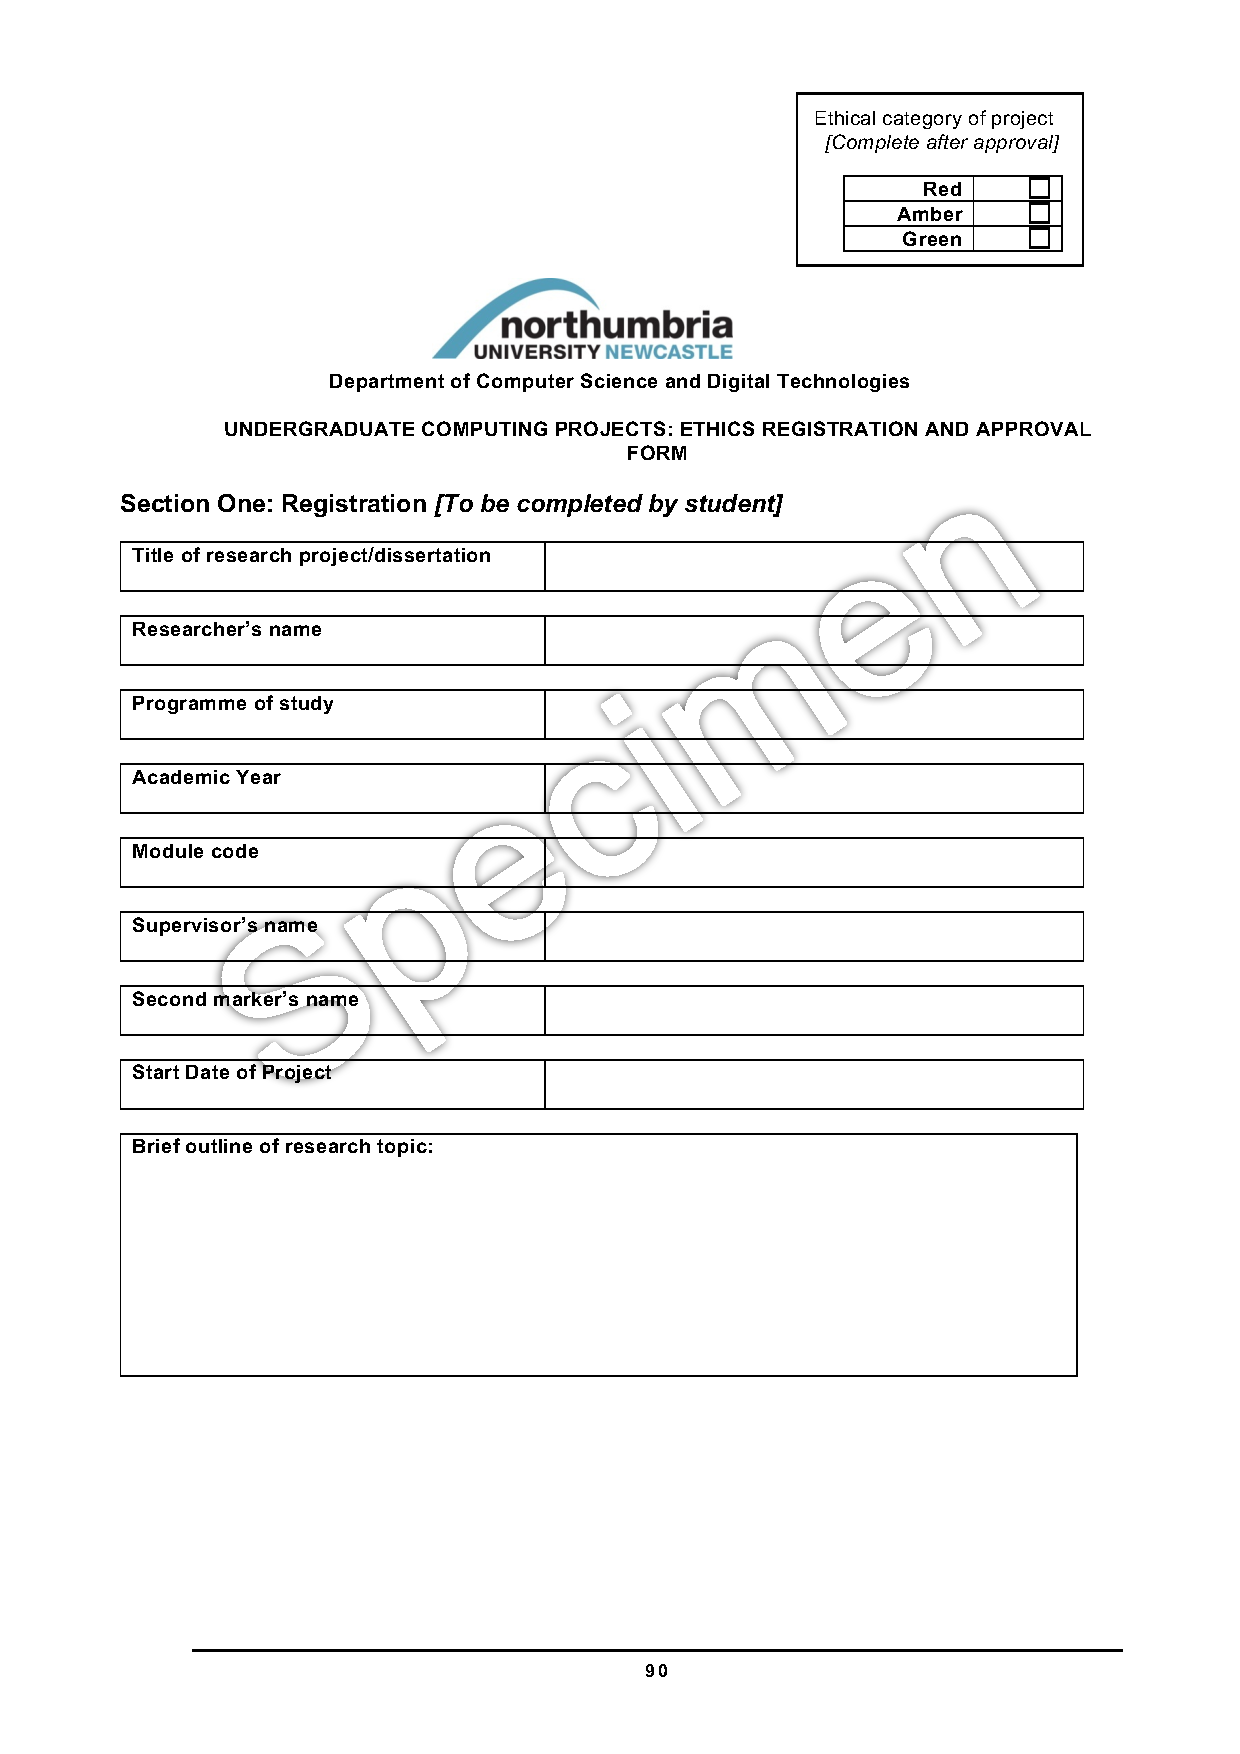
\includegraphics{ethics.pdf}
\end{tcblisting}
Assuming of course you have saved the form  as \path{ethics.pdf}

\section{Risk Assessment Form}
Likewise you can scan and include the Risk Assessment Form
\begin{tcblisting}{listing only}
\includegraphics{risk-assesment.pdf}
\end{tcblisting}

\end{document}
